\chapter{Konzeption}

In diesem Kapitel wird die Konzeption dieses Projektes bezogen auf zwei Aspekte thematisiert, nämlich Learning Management System (LMS) und WebVR, Vorbereitung einer Infusion mit WebVR.

Beim Learning Managment System (LMS) und WebVR wird erst die Konzeption des Unterrichts auf LMS beschrieben. VR-Training wird als eine Lernmethode in diesem Unterricht eingefügt.

Um die geeignete VR Technik mit LMS zu verbinden, werden native VR Applikationen mit WebVR Applikationen verglichen. Laut Ergebnis des Vergleichs fällt die Entscheidung auf die WebVR Technik.

Die WebVR Applikation kann auf drei Arten mit LMS verbunden werden. Diese werden miteinander verglichen und eine davon wird in diesem Projekt eingesetzt.

Bei der Vorbereitung einer Infusion mit WebVR werden die WebVR Applikation von vier Aspekten vorgestellt, Graphical user interface (GUI), Interaktion, Geräusche und Anordnung. Dadurch werden die sechs Kategorien der Immersion \citep{28} konkretisiert.

Graphical user interface (GUI) beschreibt die simulierte VR Umgebung. Das ist die Grundlage, sodass die praktische Übung ohne echte Materialien ausgeführt werden kann.

Interaktion beschreibt, wie die Nutzer die virtuelle Welt beeinflussen können. Denn ein Ziel des Projektes ist, eine cross-plattform darzustellen und thematisiert, wie die Interaktionen auf unterschiedlichen Geräte auszusehen hat.

Auditive Wahrnehmung hilft den Nutzern genauso wie die visuelle Wahrnehmung, die Umgebung und Objekt zu erforschen und wahrzunehmen. Bei Geräuschen geht es nicht nur um die lebendige VR Umgebung, sondern auch um das Feedback der Interaktion.

Als eine Übung für Pflege-Studenten müssen die richtige und fachliche Handlungen vermittelt werden. Da es in der echten Welt aber unzählbar viele Interaktionsmöglichkeiten gibt, wird sich in der VR Umgebung auf einige ausgewählte Aktionen beschränkt und geleitet. Bei Anordnung werden die Methoden erzählt, um die effektive Übung reibungslos durchzuführen. 

\section{Learning Managment System (LMS) und WebVR}
Laut der Forschung ist die Lernmethode entscheidend für den Lerneffekt. WebVR Technik bietet die neue Möglichkeit, neue Lernmethoden, wie beispielsweise VR-Training zu entwickeln. Hier wird eine Konzeption eines mit VR-Training verbundenen Unterrichts auf LMS beschrieben.

 \subsection{Erstellung eines Unterrichts}
 Das VR-Training ist eine neue Lernmethode für das Lernen, besonders für praktische Übung. Vor der Durchführung einer Übung soll genügend Vorwissen angeboten werden. Deswegen wird erst eine Unterrichtseinheit auf dem Learning Managment System erstellt.

 Laut der Erklärung im Kapitel Stand der Forschung \glqq Multisensorische und emotionale Wahrnehmungen können die Gedächtnisleistung verstärken\grqq\ \citep{11} sollen die Lernmaterialien des Unterrichts vielfältig sein. Durch vier Lernmaterialien in drei Arten wird das Vorwissen angeboten:
 \begin{enumerate}
    \item Text: Text ist das traditionelle Lernmaterial. Es spielt eine unersetzbare Rolle im Lernprozess. Die Lesegeschwindigkeit kann der Lernende individuell bestimmen. Während des Lesens kann der Leser gut nachdenken, sich Dinge merken und gegebenenfalls notieren.
    \item Video: Video ist ein intuitives Lernmaterial. Zwei Wahrnehmungen, Sehen und Hören werden aufgerufen, wenn man ein Video anschaut. Durch ein Video kann die Handlung sehr konkret gezeigt werden. Zur Zeit ist Video das beste und am meisten verbreitete Medium, praktische Kenntnisse zu vermitteln.
    \item Diagramm: Diagramm ist eine optimale Darstellung für Strukturen und Sequenzen. Die deutlichen, meist abstrakten, visuellen Zeichnungen sind hilfreich für das Verständnis und für das dauerhafte Merken eines Ablaufes.
 \end{enumerate}

 Nach der Sammlung der Vorkenntnisse können die Lernenden durch den Zugang in diesem Unterricht in VR Umgebung reingehen, um die praktische Übung durchzuführen. In der VR Umgebung steht das Vorwissen als Hinweise auf einem Whiteboard zu Verfügung. Die Hinweise können von den Lernenden ignoriert werden, wenn die Lernenden die Übung auch alleine flüssig schaffen können. Allerdings sollen die Hinweise einfach zu erreichen sein, damit der Lernende nicht aus VR Umgebung herausgehen muss, um Hilfsmittel zu suchen, wenn sie sich nicht an die Vorkenntnisse erinnern können. Wenn die Übung geschafft wird, können die Lernenden wieder zu dem Unterricht geleitet werden.

 Nach der Übung wird ein Test angeboten, um das Ergebnis des Lernens zu prüfen. Das Ergebnis des Tests wird in Learning Managment System gespeichert und als Feedback an die jeweilige Lehrperson geschickt. (Abbildung ~\ref{fig:moodleBeispiel})
 
\begin{figure}[ht]
\vspace*{0.2cm}
\centering
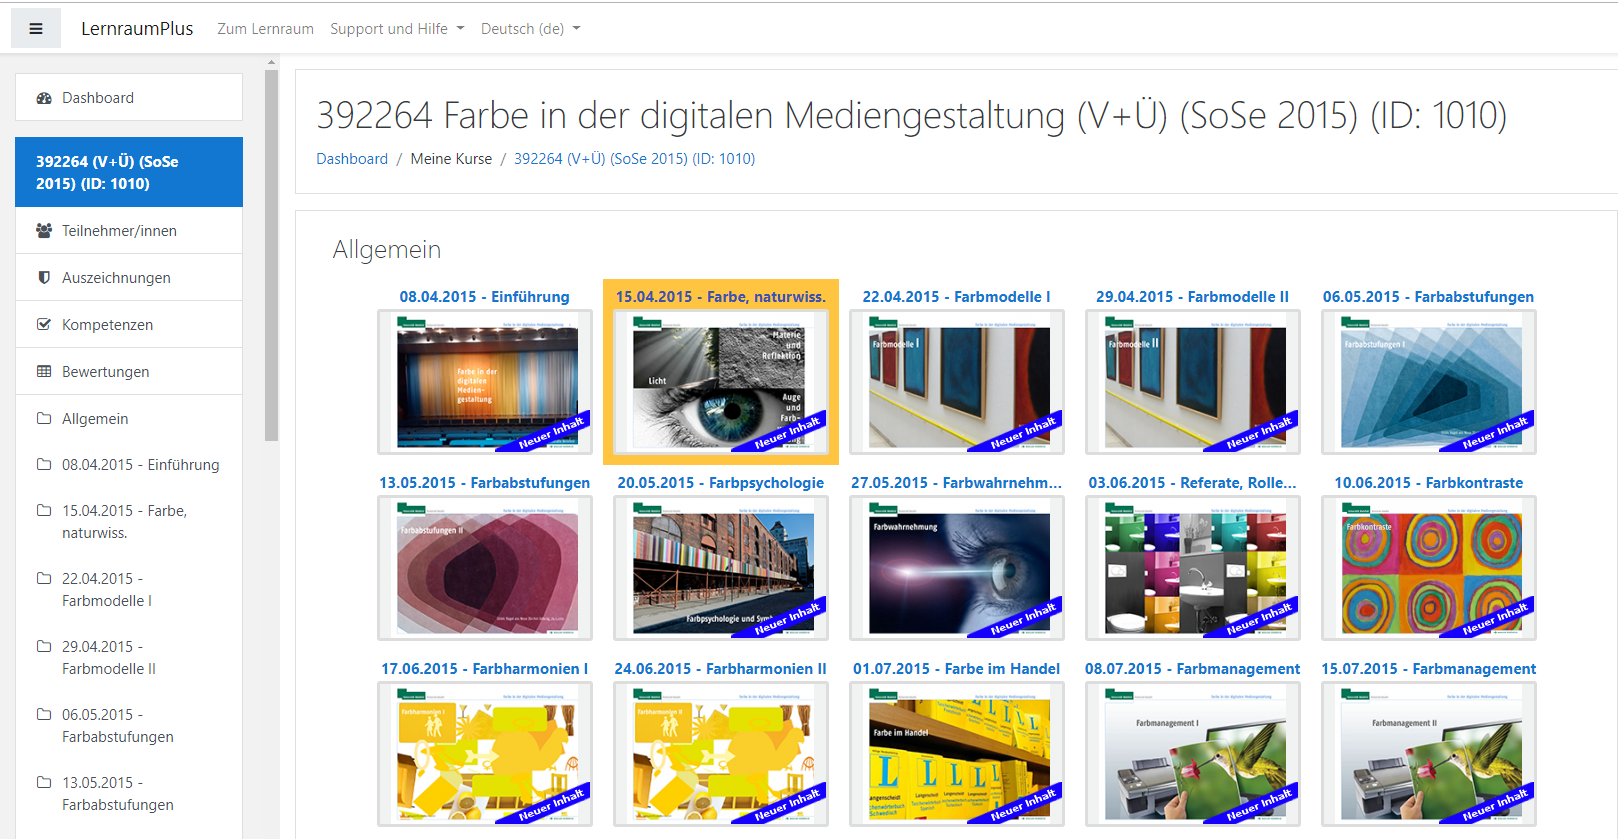
\includegraphics[width=\textwidth]{images/moodleBeispiel.png}
\caption{Moodle}
\label{fig:moodleBeispiel} 
\end{figure}

 \subsection{WebVR}
 Zwei Ziele des Projekts haben höchste Priorität: gute Erreichbarkeit und Verbindung mit LMS.

 Der größte Vorteil der nativen Apps bezüglich der Erreichbarkeit ist die Möglichkeit der offline-Nutzung. Wenn die Applikation installiert ist, ist während der Nutzung der VR Übung kein online Zugang notwendig. Allerdings erfordert die Installation eine hohe Rechner-Kapazität (oder Smartphone-Kapazität). Wenn viele Übungen werden in eine Applikation eingepackt, führt es zu Missbrauch der Kapazität, weil tatsächlich die geschaffte Übungen nicht gebraucht sind. Wenn jede Übung eigene Applikation hat, wird viel extra Zeit in Installation vor dem Lernen investiert, sodass der Vorteil der offline Erreichbarkeit nicht mehr existiert.

 Capterra ist eine Webseite, die deren Benutzern hilft, geeignete Software in unterschiedlichen Bereichen zu finden. Es werden insgesamt 432 Softwares gefunden, wenn \glqq LMS Software \grqq\ gesucht wird. 406 von 432 der gefundenen LMSs haben web basierte Applikation zu Verfügung. Das heißt, dass 94\% LMS Internet fordert und können in Browser laufen lassen.

 WebVR Applikation wird auch im Browser aufgerufen. Ohne Software Wechseln wird zu keiner Ablenkung geführt. Außerdem ist die Schnittstelle zwischen Web Applikationen einfacher zu implementieren, deswegen ist die Verbindung zwischen LMS und WebVR barrierefrei. Darüber hinaus fordert LMS sowieso Internet, kann die Anforderung für Internet von WebVR nicht als Nachteil gelten. 

 Laut der oben genannten Gründe wird für die WebVR Technik entschieden, die VR Übung für den Vorbereitung einer Infusion zu realisieren.

 \subsection{Verbindung zwischen WebVR Applikation und Learning Managment System}
 Es gibt drei Formen für die Verbindung (Abbildung ~\ref{fig:formenderVerbindung}) zwischen WebVR Applikation und Learning Managment System (LMS):
 \begin{enumerate}
   \item WebVR Applikation neben dem Learning Managment System:
     \subitem In LMS wird der Zugang zur VR Umgebung geboten und durch URL können Informationen in VR Umgebung miteingebracht werden. In VR Umgebung kann auch der Zugang zurück zu LMS geboten werden. Aber keine Information kann von VR Umgebung an LMS übermittelt werden.
     
     Der Vorteil ist, dass die WebVR Applikation unabhängig von LMS ist. Die WebVR Applikationen müssen nicht für ein bestimmtes LMS konfiguriert werden. Das heißt, dass jede LMS mit solcher WebVR Applikation verbunden werden kann.
     
     Der Nachteil ist, dass der Austausch der Informationen zwischen WebVR Applikation und LMS einspurig ist. Das LMS kann Keine Information von WebVR Applikation bekommen. Außerdem muss jede Änderung in WebVR Applikation (z.B. Umschreibung der Hinweise) von einem Programmierer gemacht werden, der in das Projekt eingearbeitet ist. Der Lehrende ist nicht in der Lage, alleine die Übung zu verbessern oder zu korrigieren.
     
   \item WebVR Applikation teilweise in dem Learning Managment System:
     \subitem In LMS wird der Zugang zur VR Umgebung geboten, allerdings ist der Zugang keine URL, sondern erfahrungsmäßig ein Plugin. Durch das Plugin kann die WebVR Applikation die versteckten zugänglichen Daten der Datenbank des Unterrichts bekommen. Mit dem Zugang der Datenbank ist die WebVR Applikation in der Lage, die Daten in einer Datenbank zu speichern und die Daten aus der Datenbank zu lesen. Durch das Middleware wird die gegenseitige/zweispurige Kommunikation zwischen WebVR Applikation und LMS ermöglicht. Obwohl durch URL die zugänglichen Daten auch übertragen werden können, ist es sehr unsicher für das LMS, weil die URL öffentlich ist.
     
     Der Vorteil ist, dass die Kommunikation zwischen WebVR Applikation und LMS frei ist. Das heißt, dass die Übertragung nicht nur für Text sondern auch für Bild, Audio und Video ermöglicht ist, und dass LMS die Informationen, die während der Übung in WebVR Applikation erstellt werden, ohne zeitlichen Verzug bekommen kann. Darüber hinaus kann der Lehrende durch dem Plugin die Inhalte in WebVR Applikation direkt teilweise verändern.
     
     Die Nachteile sind, dass die WebVR Applikation von dem LMS abhängig ist und die Entwicklung aufwendig ist. Um die Daten barrierefrei zu übertragen, muss eine entsprechende Schnittstelle in WebVR Applikation konfiguriert werden. Bei der Entwicklung werden nicht nur WebVR Applikation, sondern auch das Plugin von LMS geschrieben. Zusätzlich wird eine entsprechende Datenbank eingerichtet.
     
   \item Learning Management System in WebVR Applikation
     \subitem Bei dieser Form ist die Methode der Kommunikation zwischen WebVR Applikation und LMS ähnlich zu der zweiten Form. Der größte Unterschied liegt an der Nutzererfahrung. Die Graphical User Interface des LMS wird in der VR Umgebung dargestellt. Das heißt, dass von Anfang an der Lernende in der VR Umgebung steht. In der VR Umgebung wird Vorwissen gesammelt, praktische Übung durchgeführt und am Ende ein Test durchgeführt.
     
     Der Vorteil ist, dass der ganze Lernprozess in VR Umgebung integriert wird und keine Ablenkung von außen existiert (zumindest keine visuelle Ablenkung).
     
     Die Nachteile sind dabei aber die aufwendige Entwicklung und Lesen eines Textes in einer ungewöhnlichen Umgebung. Um die Inhalte in LMS logisch und effektiver darzustellen, müssen geeignete graphische Komponenten in der VR Umgebung gestaltet und implementiert werden. Es gibt noch kein bestimmtes Ergebnis einer Forschung, ob das Lesen einer Textes in einer virtuellen Umgebung den gleichen Effekt wie das Lesen auf Papier ergibt. Allerdings muss es erst angewöhnt werden, mit keinem konkreten Medium in der Hand zu lesen.
 \end{enumerate}
 
\begin{figure}[ht]
\vspace*{0.2cm}
\centering
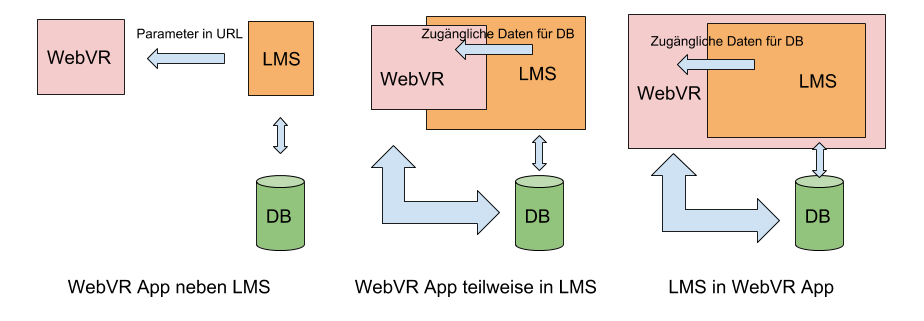
\includegraphics[width=\textwidth]{images/formenderVerbindung.png}
\caption{Formen der Verbindung}
\label{fig:formenderVerbindung} 
\end{figure}

Bei diesem Projekt wird die erste Form implementiert. Wegen der begrenzten Entwicklungszeit werden die zweite und dritte Formen bei diesem Projekt nicht realisiert.

\section{Vorbereitung einer Infusion mit WebVR}

Als Schwerpunkt des Projektes wird die Konzeption der Übungsvorbereitung einer Infusion mit WebVR ausführlich erklärt. Die Konzeption wird nach den Kategorien der Immersion von Jason Jerald\citep{28} aufgebaut.

 \subsection{Graphical user interface (GUI)}
 GUI ist die visuelle Darstellung einer Applikation. Für dieses Projekt gilt GUI als die simulierte Umgebung. Laut der Forschung führt eine lebendigere Simulation zu besserem Behalten von Informationen bei VR-Training. \citep{27} Die Kategorien Extensiveness, Surroundness und Vividness werden durch die GUI realisiert.
 
  \subsubsection{Szene}
  Die VR Umgebung bezieht sich auf das \glqq Skillslab\grqq\ der Fachhochschule Bielefeld. Um die relevanten Objekte der Übung hervorzuheben, wird die Szene vereinfacht. (Abbildung ~\ref{fig:realToPrototype})
  
\begin{figure}[ht]
\vspace*{0.2cm}
\centering
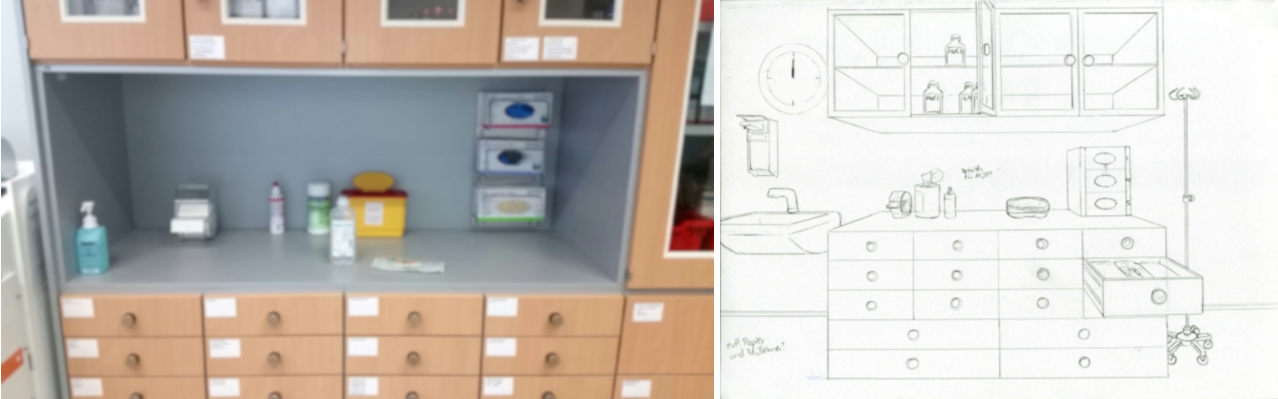
\includegraphics[width=\textwidth]{images/realToPrototype.png}
\caption{Reales Skillslab \& Prototyp}
\label{fig:realToPrototype} 
\end{figure}
  
  Der Aufbau der Szene basiert auf einem Projekt, das im Jahr 2016 entwickelt wurde\citep{26}. Die Modelle werden korrigiert und ausgebessert. (Abbildung ~\ref{fig:WithoutGlass})

\begin{figure}[ht]
\vspace*{0.2cm}
\centering
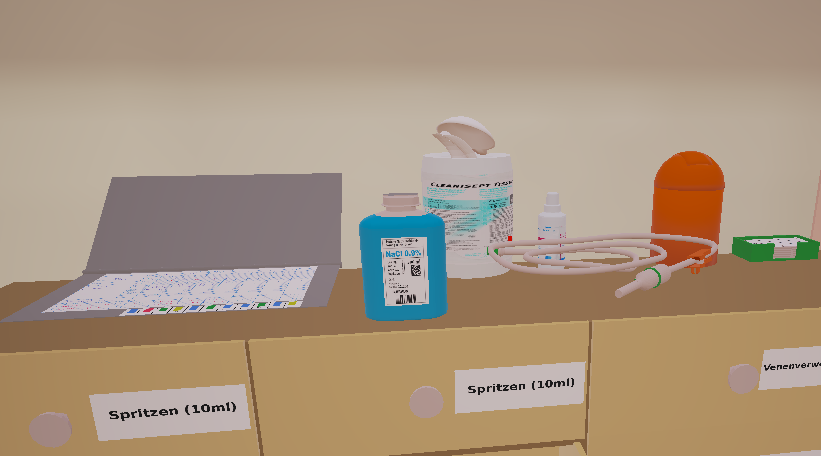
\includegraphics[width=\textwidth]{images/WithoutGlass.png}
\caption{Gear VR Version in 2016}
\label{fig:WithoutGlass} 
\end{figure}
  
   \subsubsection{lebendige Texturen}
   
   Um den Anspruch der Leistung des Smartphones zu verringern, wurden in dem damaligen Projekt unnötige Texturen nicht benutzt. Zurzeit besitzen Smartphone eine stärkere Leistung, deshalb können die Modelle mit lebhafteren Texturen gerendert werden, um die \glqq Vividness\grqq\ zu verbessern.
   
   Beispielsweise werden die wichtigsten Texturen aufgelistet:
   \begin{itemize}
       \item \textbf{Holz}: Hängeschränke, Schubladenschränke und Boden
       \item \textbf{Metal}: Griffe der Hängeschränke und Schubladenschränke, Handschuh-Spender und Infusionsständer
       \item \textbf{farbiges Plastik}: Kanülen-Sammler, Mülleimer, Spenderbox, Armhebelspender usw.
       \item \textbf{Wand}: Wände und Decke
   \end{itemize}
   
   \subsubsection{Transparenz}
   Objekte mit eigentlich transparenten Materialien, wie beispielsweise Infusionsflasche und Infusionsbesteck, wurden im Jahr 2016 versuchshalber mit durchsichtigen Materialien ausgestattet. Allerdings wurden die transparenten Materialien nicht richtig in Gear VR dargestellt. Vermutlicher war dabei der Grund, dass die Leistung der damaligen Smartphones zu schwach war, weil die Renderung der transparenten Objekten sehr aufwendig ist.
   
   Im Jahr 2018 ist die Leistung der Smartphones schon viel stärker. Es sollte möglich sein, in diesem Projekt die transparenten Objekten zutreffend zu rendern.
   
   \subsubsection{Modell Korrektur von Kanülen-Sammler}
   Im Jahr 2016 wurde ein medizinisch fachlicher Fehler bei der Modellierung gemacht: der Kanülen-Sammler wurde als normaler Mülleimer modelliert und somit nicht korrekt dargestellt. Ein Kanülen-Sammler ist einmalig verschließbar, bzw ist schwierig, zu öffnen, sobald dieser einmal geschlossen wurde. Im Gegensatz dazu ist der Deckel eines normalen Mülleimers sehr locker und beweglich, und lässt sich unendlich oft öffnen und schließen. Diese Öffnungsmöglichkeiten eines herkömmlichen Mülleimers ziehen viele Risiken mit sich, da gebrauchte Spritzen herausfallen könnten. (Abbildung ~\ref{fig:muelleimerKanueleSammler})

\begin{figure}[ht]
\vspace*{0.2cm}
\centering
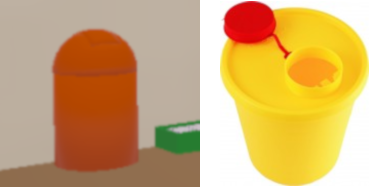
\includegraphics[width=\textwidth]{images/muelleimerKanueleSammler.png}
\caption{Mülleimer \& Kanüle Sammler}
\label{fig:muelleimerKanueleSammler} 
\end{figure}

In diesem Projekt wurde die fehlerhafte Modellierung ausgebessert, sodass nun anstelle einer Mülleimers, ein Kanülen-Sammler in der vurtuellen Umgebung zur Verfügung steht.

   \subsubsection{Entfernung der Hinweis Streifen}
   Bei der Version aus dem Jahre 2016 wurde für das Feedback eine schwarze Text-Leiste am unteren Sichtfeld des Nutzers positioniert. (Abbildung ~\ref{fig:Schritt_4_2}) Feedback kam dabei in Form von Text, also Hinweisen, und gegebenenfalls mit entsprechenden Icons (dass der Nutzer beispielsweise im Besitz eines Desinfektionstuchs ist). Bei der Evaluation stellte sich heraus, dass die Hinweise nicht gut gelesen werden konnten, weil die Leiste etwas zu niedrig positioniert worden war. Eine höhere Positionierung der Text-Leiste hätte hingegen eine zu große Einschränkung des Sichtfeldes mit sich gebracht.
   
   Um die Text-Leiste \glqq verlustfrei\grqq (keine der Aufgaben, die die Leiste übernommen hat, soll vernachlässigt werden) zu entfernen, müssen erst die Aufgaben spezifiziert werden, die sie übernommen hat, sodass diese Aufgaben andere Bereiche übernehmen können und somit kein Verlust an Feedback entsteht. Insgesamt werden drei Aufgaben ermittelt:
   
   \begin{itemize}
       \item \textbf{Hinweise}: Die Aufgabe, Hinweise darzustellen wird von dem Whiteboard auf der linken Seite des Raums übernommen.
       \item \textbf{Symbol von Desinfektionstuch}: Auf PC, Smartphone und Gear VR Version wird das Modell von dem Desinfektionstuch auf der Arbeitsfläche gelegt. Auf der Vive Version kann das Desinfektionstuch direkt in Hand genommen werden. Deshalb ist das Symbol eines Deinfektionstuch nicht mehr nötig.
       \item \textbf{Symbol von Einmalhandschuhe}: Auf PC, Smartphone und Gear VR Version wird das Modell von Einmalhandschuhe direkt auf die Sicht hängt. Es bewegt sich entsprechend der Bewegung der Kamera. Auf der Vive Version wird die Modell von Händen mit Einmalhandschuhen in der hell blauer Farbe dargestellt. Deswegen ist das Symbol von Einmalhandschuhen auch nicht mehr nötig. 
   \end{itemize}
   
   Mit diesen drei Lösungen werden alle drei zugehörigen Aufgaben übernommen, sodass die schwarze Text-Leiste nicht mehr gebraucht wird und ohne einhergehende Verlüste entfernt werden kann.
   
\begin{figure}[ht]
\vspace*{0.2cm}
\centering
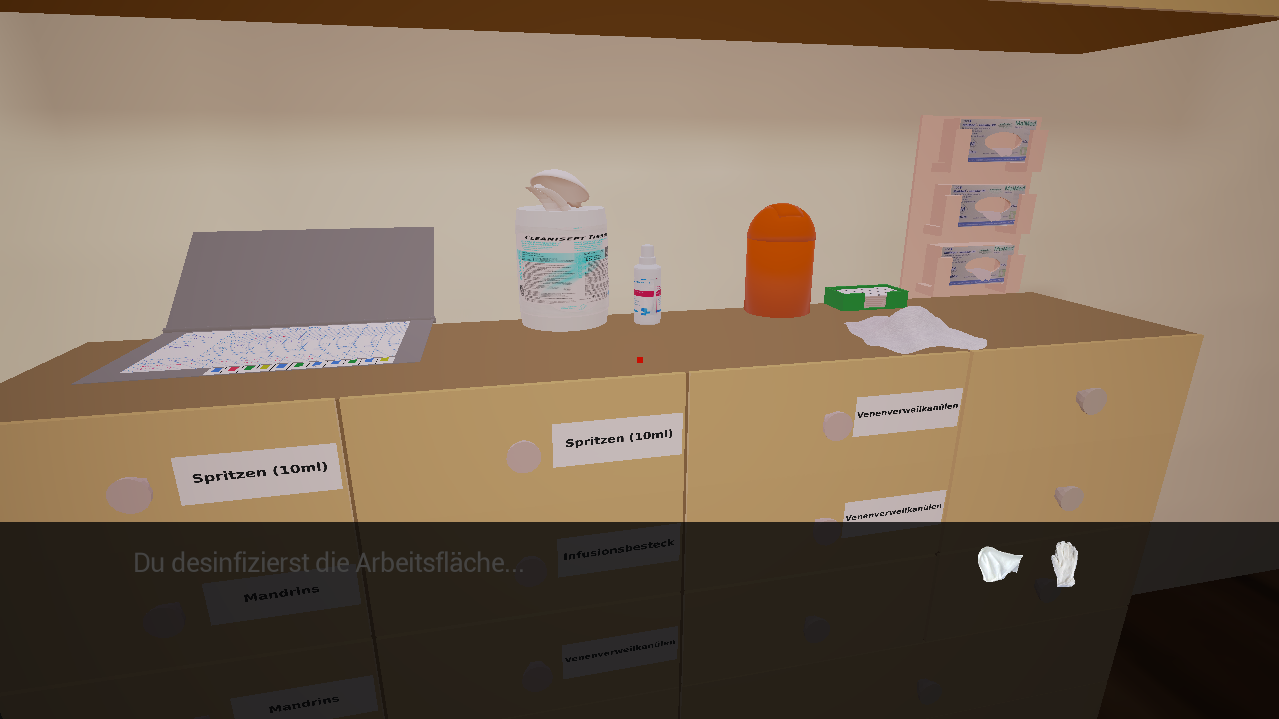
\includegraphics[width=\textwidth]{images/Schritt_4_2.png}
\caption{Szene mit Text-Leiste}
\label{fig:Schritt_4_2} 
\end{figure}
   

   \subsubsection{Modellierung der Hände}
   Auf der Vive Version können die Objekte mit dem Controller genommen werden. Die Controller übernehmen die Rolle von Händen, deswegen sollen entsprechende Modelle der Händen die Modelle der Vive Controllers in der VR Umgebung ersetzen.
   
   Die Modelle der Händen sollen sich je nach der Aktion der Controller in ihrer Haltung verändern. Wenn der Auslöser (TODO: meinst du den Hair-Trigger?) gedrückt wird, soll die entsprechende Hand leicht zu einer Faust geballt werden. Wenn der Auslöser hingegen losgelassen wird, soll die Faust wieder gelöst werden.

 \subsection{Interaktion}
 Interaktion ist ein wichtiger Teil der WebVR Applikation, weil die nicht nur die Implementierung von \glqq Interactability\grqq ist, sondern auch enge Beziehung mit \glqq Matching\grqq hat.
 
 Um bessere Benutzererfahrung zu haben, soll die Interaktionen auf der einen Seite die Merkmale der unterschiedlichen Geräte möglichst geeignet und in voller Ausprägung benutzen, auf der anderen Seite nicht zu vielfältig sein, sodass der Fokus nicht auf dem Lernen der Interaktion bzw dem Händeln des Geräts liegt. 
 
 Da die WebVR Applikation cross-plattform ist, werden die Konzeptionen der Interaktion nach den Typen der Geräte gliedert. (Tabelle ~\ref{tab:Interaktionen})

 Für jedes Geräte wird von drei Aspekten der Interaktionen erklärt:
 
 \textbf{Exploration}: Änderung der Sicht. Aspekt (TODO: ich weiß nicht genau was du mit "Aspekt" meinst... vllt lieber "Erforschen der virtuellen Umgebung"? "Umsehen", "sich mit der Umgebung vertraut machen"; frag da am besten Thies, was du statt Aspekt schreiben kannst).
 
 \textbf{Navigation}: Translation der Kamera.
 
 \textbf{Manipulation}: Aktivierung der Aktivität des Objektes für PC, Smartphone und Samsung Gear VR, zusätzlich Überprüfung, Greifen und Befreiung für HTC Vive.

 \subsubsection{PC}
 Ein PC ist ein wichtiges Produktivitätswerkzeug für alle Menschen. Im Vergleich zum Smartphone hat ein PC bessere Leistungen und einen größeren Bildschirm. Im Bereich E-Learning hat PC noch größere Vorteile bei der Eingabe, deswegen spielen PCs eine unersetzbare Rolle bei E-Learning. Durch die WebVR Technik kann die VR Umgebung auf flachen Bildschirmen gezeigt werden, damit wird die Erreichbarkeit der VR Applikation sehr verbessert. 
 
  \textbf{Exploration}
  
  Um die VR Umgebung zu explorieren, wird den Aspekt verändert. Der Aspekt ist die Sicht, die in Kamera aufgenommen ist, nämlich die Sicht des Benutzers. Die Bewegung des Blickfeldes erfolgt mit der Bewegung der Maus. Es gibt zwei Varianten, um die Bewegung des Aspekts zu bestimmen.
  
  Eine Variante ist, dass die Bewegung des Aspekts durchgeführt wird, wenn die Maus sich bewegt und deren linke Taste der Maus gedrückt wird. Wenn die linke Taste losgelassen wird, bewegt sich der Aspekt nicht. Der Vorteil ist, dass eine solche Interaktion ähnlich zu alltäglichen Applikationen ist, wie beispielsweise Google Maps. Dadurch bestehen gute Chancen, dass sich Nutzer schnell mit der Interaktion vertraut machen. Der Nachteil ist, dass eine Aktivität durch zwei Aktionen, Maus Druck und Maus Bewegung, aufgerufen wird. Das macht die Interaktion kompliziert, wenn der Aspekt sich häufig bewegt.
  
  Die andere Variante ist, dass die Bewegung Mode aktiviert wird. Das heißt, dass der Aspekt sich solange nach der Maus bewegt, bis ESC Taste gedrückt wird. Der Vorteil ist, dass die Interaktion einfach ist, und der Druck auf die Maus verringert wird. Der Nachteil ist, dass der Mauszeiger während der Bewegung Mode verschwindet. Es könnte passiert, dass der Benutzer die Maus viel herum schwenkt, um den Mauszeiger zu finden, sodass der Aspekt auch sehr viel hin und her wackelt.
  
  Die verwirrende Aktivität bei der zweite Variante passiert normalerweise nur bei der erstmaligen Nutzung und ist "harmlos". Allerdings der Vorteil davon ist eindeutig. Deshalb wird die zweite Variante implementiert.
  
  \textbf{Navigation}
  
  Die Position der Kamera ist der Ort, wo der Nutzer in der VR Umgebung steht. Die Translation der Kamera führt zur Navigation des Nutzers in dem simulierten Raum. Zwei Möglichkeiten der Navigation werden geboten, eine automatische und eine manuelle.
  
  Automatische Navigation bedeutet, dass die Kamera sich automatisch zu einem Ort bewegt, wenn die Translation zu einer besseren Benutzererfahrung führt. Die Ziele sind, den Benutzer zu leiten, Objekte zu betrachten und die Genauigkeit zu erhöhen, wenn der Nutzer mit einem kleinen Objekt interagieren will. Zum Beispiel soll das Plakat über die Händedesinfektion während der Desinfektion gut betrachtet werden können, deswegen bewegt sich die Kamera automatisch zu dem Plakat, wenn der Nutzer Hände desinfizieren will. Ein anderes Beispiel ist, dass die Kamera automatisch dem Infusionsbesteck näher kommt, wenn der Nutzer das Rädchen des Infusionsbestecks drehen will.

  Neben der automatischen Bewegung kann die Kamera zudem durch Druck auf den Tasten W, A, S, D navigieren. Das bietet die Freiheit, sich in der VR Umgebung umzuschauen. Ohne die manuelle Navigation kann die Übung auch barrierefrei durchgeführt werden.
  
  \textbf{Manipulation}
  
  Die Manipulation wird mit dem Zeiger ausgeführt. Der Zeiger ist ein schwarzer Ring, der immer in der Mittel der Sicht der Kamera steht. Der ist zuständig für den Aufruf einer möglichen Aktion eines Objekts, auf das dieser zeigt.
  
  Wenn der Benutzer mit dem nächsten Objekt hinter dem Zeiger interagieren kann, wechselt die Farbe des Rings zu grün, um dem Nutzer so zu symbolisieren, dass eine Aktion möglicht ist. Allerdings bedeutet der grüne Zeiger nicht, dass die Aktion des Objekts die korrekte ist. Die Übung wird in einer bestimmtem Reihenfolge durchgeführt, wenn eine Aktion eigentlich noch nicht dran ist, gilt das Auslösen dieser Aktion als Fehler.
  
  Wenn der Zeiger grün ist und die linke Taste der Maus gedrückt wird, scheint die Farbe des Zeigers rot für ca. 0,3 Sekunden, um die Botschaft an dem Benutzer geben, dass der Befehl, mit einem Objekt zu interagieren, ausgeführt ist. 
  
 \subsubsection{Smartphone}
 Laut der Forschung ist Mobilität ein wichtiger Trend von E-Learning. Ein wichtiger Faktor ist, dass die Mobilität des Smartphones unschlagbar ist. Smartphone bietet die Möglichkeit, in kurzem Zeitraum und im Verkehr zu lernen. Durch die WebVR Technik wird auch Smartphone unterstützt, VR Umgebung darzustellen.
 
  \textbf{Exploration}
  
  Zwei Methoden werden für Exploration angeboten, um unterschiedliche Situation anzupassen.
  
  Die intuitive Methode ist, das Smartphone zu bewegen. Die simulierte Umgebung wird im Smartphone räumlich dargestellt. Aber aufgrund der Begrenzung des Bildschirms ist nur der Raum teilweise im Blickwinkel. Durch die Bewegung des Smartphones werden andere Ort in dem Raum gesehen. (Abbildung ~\ref{fig:paperPrototypewiths8mini})

\begin{figure}[ht]
\vspace*{0.2cm}
\centering
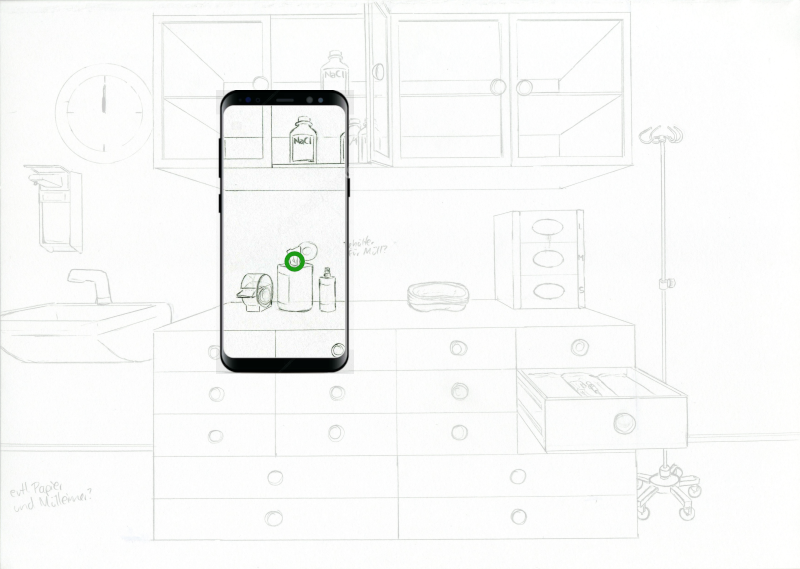
\includegraphics[width=\textwidth]{images/paperPrototypewiths8mini.png}
\caption{Smartphone Prototyp}
\label{fig:paperPrototypewiths8mini} 
\end{figure}

  Es ist unvermeidbar, den Körper zu drehen, um seitlich gelegene Objekt zu sehen, wenn man mit der ersten Methode das Smartphone bewegt. Allerdings ist es unmöglich, es um einen größeren Winkel zu drehen, wenn man auf einem Stuhl sitzt. Außerdem beeinflusst es andere Leute, wenn man in der Öffentlichkeit (beispielsweise in einer Bibliothek) solch große Bewegungen macht. Um dieses Probleme zu lösen, wird die zweite Methode angeboten, dass der Aspekt durch das Wischen auf dem Bildschirm verändert wird. Obwohl diese Methode nicht so intuitiv wie die erste Methode ist, vermehren sich dadurch die Einsatzmöglichkeiten.
  
  \textbf{Navigation}
  
  Das Smartphone bietet nur 3DoF Erkennung, nämlich Rotation. Deswegen kann die Translation der Kamera nicht mit der Translation des Smartphones verbunden werden. Um ein Objekt genauer anzuschauen und Interaktion zu vereinfachen, wird eine automatische Navigation wie auf dem Laptop angeboten.
  
  \textbf{Manipulation}
  
  Der Form des Zeigers ist die gleich wie auf dem Laptop. Da auf einem Smartphone keine Maus zu Verfügung steht, wird die Bestätigung des Zeigers durch \glqq Anstarren\grqq\ (eng. gaze) ausgeführt. Wenn der Zeiger ca. 0,5 Sekunde auf einem Objekt verharrt, wird dadurch die Aktion des jeweiligen Objecktes initiiert.
  
 \subsubsection{Samsung Gear VR}
 Samsung Gear VR ist ein gut verbreitetes mobile HMD im Markt. Es ist ein typisch 3Dof HMD. Gear VR kann mit oder ohne Controller benutzt werden.
 
  \textbf{Exploration}
  
  Durch Gear VR wird der Benutzer in dem simulierten virtuellen Raum hineinversetzt. Die Exploration wird durch der Rotation des Kopfes durchgeführt, ähnlich wie im realen Leben. Allerdings wird nur Rotation von HMD erkannt, weil Gear VR 3DoF ist.
  
  \textbf{Navigation}
  
  \textsl{Ohne Controller}:
  
  Wenn Gear VR ohne Controller ist, kann es als Google Cardboard gelten. Die Navigation ist die gleiche wie die Navigation mit Smartphone, nur dass automatische Navigation angeboten wird.
 
  \textsl{Mit Controller}: (Abbildung ~\ref{fig:gearViveController})
  
  Der Gear VR Controller ist ein 3DoF Controller, dass nur die Rotation erkannt wird. Es soll eine Kurve aus dem Controller ausstrahlen, die auf dem Boden landen soll, wenn das Trackpad gedrückt wird. Dort wird als der Zielort gezeichnet. Wenn den Tranlation Befehl durch der Loslösung auf dem Trackpad auf dem Gear VR Controller gesendet, soll die Kamera sich zu der gezeichneten Position navigieren.

  \textbf{Manipulation}
  
  \textsl{Ohne Controller}:
  
  Der Zeiger kann in zwei Formen dargestellt werden.
  
  Eine Möglichkeit ist, dass der Zeiger ebenso wie auf dem Laptop und dem Smartphone als Ring gezeigt wird. Der Vorteil ist, dass der Zeiger eindeutig ist. Der Ring ist auf dem komplizierten Hintergrund (die Objekten in dem Raum) einfach zu erkennen. Der Nachteil ist, dass der Treffpunkt mit den Objekte nicht klar ist, besonders wenn das Ziel sehr klein ist.
  
  Die andere Variante ist durch Raycaster. Ein Raycaster ist eine von einer bestimmten Position ausstrahlende Linie, die die durchgegangenen Objekte erkennen kann. In diesem Projekt wird das nächste Objekt zu dem Ausgangspunkt der Linie als das getroffene Objekt bezeichnet. Ein aus Augen Position ausstrahlendes Raycaster kann als der Zeiger gelten. Der Vorteil ist, dass die Position des Treffpunkts ganz genau ist. Der Nachteil ist, dass die Linie vor dem Komplizierten Hintergrund nicht stark genug hervortritt.
  
  Die Merkmale der beiden Varianten sind eindeutig. Die Entscheidung wird bei der Implementierung nach der Betrachtung des Endeffekts getroffen.
  
  Die Bestätigung des Zeigers kann durch den Druck auf das Touchpad der Gear VR oder auch durch \glqq Anstarren\grqq\ wie auf dem Smartphone durchgeführt werden.
  
  \textsl{Mit Controller}:
  
  Ein Raycaster soll aus dem Controller ausstrahlen. Durch Betätigun des Auslösers des Controllers wird versucht, die Aktion des getroffenen Objekts zu aktivieren.
  
 \subsubsection{HTC Vive}
 HTC Vive ist ein 6DoF HMD mit starker Leistung. Eine Vive wird mit einem PC verbunden. Die WebVR Applikation kann durch normale Browser wie Firefox aufgerufen und die VR Umgebung wird zeitgleich an das HMD geschickt.
 
  \textbf{Exploration}
  
  Wie mit der Gear VR wird die Bewegung des Aspekts auch durch die Bewegung des Kopfs durchgeführt. Da HTC Vive 6DoF hat, werden nicht nur die Rotation sondern auch die Translation erkannt. Somit ist die HTC Vive in der Lage, die Bewegung des Kopfs in der VR Umgebung vollständig zu simulieren.
  
  \textbf{Navigation}
  
  Auch wie mit der Gear VR strahlt eine Kurve aus dem Controller, die auf dem Boden landet, und den Zielort zu bildet, wenn das Trackpad gedrückt wird. Durch dsa Loslassen des Trackpads auf dem Controller wird die Bewegung bestätigt und durchgeführt. (Abbildung ~\ref{fig:gearViveController})
  
  \textbf{Manipulation}
  \begin{itemize}
  \item \textbf{Aktivierung der Aktion des Objektes}: Durch Drücken des Auslösers wird versucht, die Aktion des jeweiligen Objektes zu aktivieren.
  \item \textbf{Greifen}: Wenn der Controller mit einem Objekt überlappt und der Auslöser auf dem Controller gedrückt und nicht losgelassen wird, befindet sich das Objekt ab dem Zeitpunkt in der Hand (eigentlich dem Controller) Nutzers.
  \item \textbf{Loslassen}: Wenn ein Objekt in einer Hand (Controller) gehalten wird, und deren Auslöser losgelassen wird, wird das Objekt losgelassen. Das heißt, dass das Objekt entweder auf eine bestimmte Position gelegt wird oder fällt.
  \item \textbf{Überprüfung}: Wenn ein Objekt überprüft werden muss, wird ein Raycaster aus der Position der Augen ausstrahlt. Wenn der Raycaster die richtige Position trifft und der Auslöser von einer leeren Hand gedrückt wird, wird die Überprüfung durchgeführt.
  \end{itemize}

\begin{figure}[ht]
\vspace*{0.2cm}
\centering
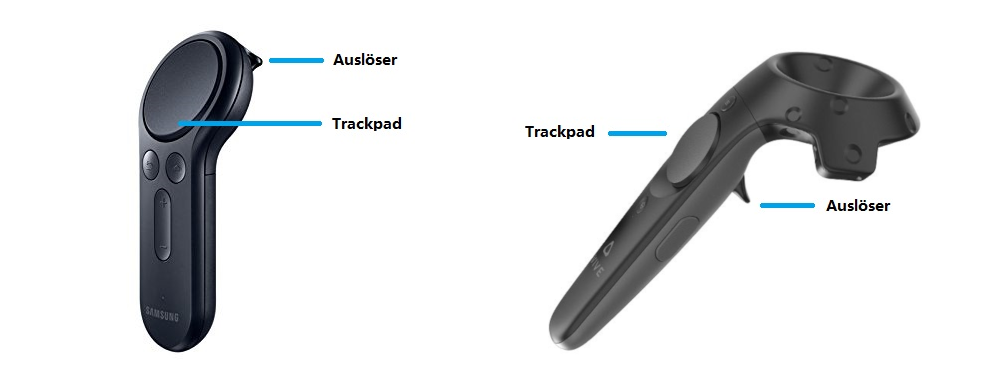
\includegraphics[width=\textwidth]{images/gearViveController.png}
\caption{Gear VR Controller \& Vive Controller}
\label{fig:gearViveController} 
\end{figure}
  
\begin{table}[ht]
\begin{tabular}{llll}
\hline
                                                                            & Exploration                                                                                                                                 & Navigation                                                                                                          & Manipulation                                                                                                                                                                                          \\ \hline
PC                                                                          & \begin{tabular}[c]{@{}l@{}}1.\\ Maus clicken\\ und bewegen\\ 2.\\ Maus clicken\\ dann bewegen\\ (ESC Tasten zu\\ deaktivieren)\end{tabular} & \begin{tabular}[c]{@{}l@{}}Manuell:\\ W,A,S,D Tasten\\ \\ drücken\\ \\ Automaticsch:\\ Objekte anschauen\end{tabular} & \begin{tabular}[c]{@{}l@{}}Aktivieren:\\ Maus clicken\end{tabular}                                                                                                                                    \\ \hline
Smartphone                                                                  & \begin{tabular}[c]{@{}l@{}}1. Smartphone\\ bewegen\\ 2. Bildschirm\\ berühren\end{tabular}                                                  & \begin{tabular}[c]{@{}l@{}}Automatisch:\\ Objekt anschauen\end{tabular}                                             & \begin{tabular}[c]{@{}l@{}}Aktivieren:\\ Objekt anstarren\end{tabular}                                                                                                                                \\ \hline
\begin{tabular}[c]{@{}l@{}}Samsung\\ Gear VR\\ ohne Controller\end{tabular} & Kopf bewegen                                                                                                                                & \begin{tabular}[c]{@{}l@{}}Automatisch:\\ Objekt anschauen\end{tabular}                                             & \begin{tabular}[c]{@{}l@{}}Aktivieren:\\ 1.\\ Touchpack clicken\\ 2.\\ Objekt anstarren\end{tabular}                                                                                                  \\ \hline
\begin{tabular}[c]{@{}l@{}}Samsung\\ Gear VR\\ mit Controller\end{tabular}  & Kopf bewegen                                                                                                                                & Trackpad clicken                                                                                                    & \begin{tabular}[c]{@{}l@{}}Aktivieren:\\ Auslöser clicken\end{tabular}                                                                                                                                \\ \hline
HTC Vive                                                                    & Kopf bewegen                                                                                                                                & Trackpad clicken                                                                                                    & \begin{tabular}[c]{@{}l@{}}Aktivieren:\\ Auslöser betätigen\\ \\ Greifen:\\ Auslöser drücken\\ \\ Befreien:\\ Auslöser loslösen\\ \\ Überprüfen:\\ Objekt anstarren\\ und Auslöser clicken\end{tabular} \\ \hline
\end{tabular}
\caption{Interaktionen für unterschiedlichen Geräten}
\label{tab:Interaktionen}
\end{table}

 \subsection{Geräusche}
 Die entsprechenden Geräusche können nicht nur die Lebendigkeit der VR Umgebung verstärken, sondern auch das Feedback der Interaktion verdeutlichen.
 \subsubsection{VR Umgebung}
 Um eine möglichst realitätsnahenahe VR Umgebung darzustellen, sollen erst die realen Geräusche aufgenommen werden, weil reale Geräusche die Materialien der Objekten widerspiegeln können. Die Position, wo die Geräusche erklingen, werden für jedes Objekt angepasst, da die räumliche Erkennung durch die auditive Wahrnehmung gemacht werden kann. Die Geräusche für die Objekte müssen mit der Animation synchronisiert werden, sodass die Lebendigkeit verstärkt wird.
 
 \subsubsection{Feedback der Interaktionen}
 Als ein Feedback der Interaktion spielen Geräusche eine wichtige Rolle. Die Geräusche für Interaktion sind keine realen Geräusche, sondern die Töne (Soundeffekt), die für bestimmte Interaktion geeignet sind.
 
 Insgesamt werden fünf Töne eingesetzt. Ein Ton erklingt, wenn der Zeiger auf PC, Smartphone und Gear VR ohne Controller mit Objekten interagiert. Die anderen vier Töne werden für das Drücken und Loslassen von Auslöser und Trackpad auf dem Gear VR Controller und HTC Vive Controller angepasst.
 
 \subsection{Anordnung}
 Als eine Übung soll der Ablauf nach einer korrekten Reihenfolge durchgeführt werden. Um den korrekten und fließenden Ablauf zu garantieren, wird die VR Übung von drei Aspekten gestaltet, nämlich Planung des Ablaufs, Erkennung \& Feedback der Fortschritte und Leitung des Ablaufs. Die Anordnung ist die Ausführung von Kategorie \glqq Plot\grqq.
  \subsubsection{Planung des Ablaufs}
      
  Der Ablauf wird gemäß den fachlichen Anforderungen gestaltet. Insgesamt 23 Aktivität sollen während der Übung nach richtiger Reihenfolge gemacht werden. Die Aktivitäten werden in acht Abschnitten unterteilt.
  
  \begin{enumerate}[start=0]
      \item Krankenakte überprüfen:
      
      Die Krankenakte wird von der Arbeitsfläche genommen. Die Informationen der Vorbereitung der Infusion werden gemäß der 5R-Regel (richtiger Patient, richtiges Arzneimittel, richtige Dosierung, richtige Applikationsart, richtiger Zeitpunkt) überprüft. Danach wird die Krankenakte zurückgelegt.
      
      \item Hände desinfizieren:
      
      Die Hände werden 30 Sekunden lang desinfiziert.
      
      \item Arbeitsfläche desinfizieren:
      
      Es werden die Einmalhandschuhe werden angezogen. Danach wird ein Desinfektionstuch aus der Dose herausgenommen. Anschließend wird die Arbeitsfläche desinfiziert. Die gebrauchten Einmalhandschuhe und das Desinfektionstuch werden in den Mülleimer geworfen.
      
      \item Hände desinfizieren:
      
      Die Hände werden 30 Sekunden lang desinfiziert.
      
      \item Infusionsflasche vorbereiten:
      
      Die korrekte Flasche wird aus Schrank ausgenommen. Danach werden das Etikett, der Deckel und das Medikament überprüft. Am Ende wird die Flasche auf der Arbeitsfläche abgelegt.
      
      \item Infusionsbesteck vorbereiten:
      
      Das Infusionsbesteck wird erst aus der Schublade herausgenommen. Nach der Überprüfung des Etiketts wird das Besteck auf der Arbeitsfläche abgelegt und ausgepackt. Daraufhin wird der Durchflussregler (Rollenkleme) zu gedreht und die Kappe des Dorns abgenommen. (Abbildung ~\ref{fig:infusionssystem})
      
\begin{figure}[ht]
\vspace*{0.2cm}
\centering
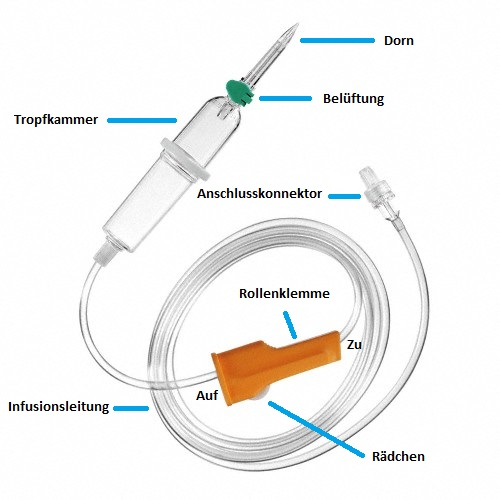
\includegraphics[width=\textwidth]{images/infusionssystem.jpg}
\caption{Infusionsbesteck}
\label{fig:infusionssystem} 
\end{figure}
      
      \item Infusion vorbereiten:
      
      Nach der Abnahmen des Deckels der Flasche wird der Dorn des Infusionsbestecks in die Flasche eingestochen. Danach wird die Flasche auf den Infusionsständer gehängt. Durch das Zusammendrücken der Tropfkammer fließt ein Teil der Frlüssigkeit in Tropfkammer. Durch die Öffnung der Rollenklemme wird die transparente Infusionsleitung mit der Flüssigkeit ausgefüllt. Am Ende wird die Infusionsleitung an der entsprechenden Vorrichtung befestigt.
      
      \item Namenetikett vorbereiten:
      
      Nach der Beschriftung eines Etiketts/Aufklebers wird dieses auf die Flasche geklebt.
      
  \end{enumerate}
  
  Die Abschnitte sind nicht nur die abstrakte Gliederung, sondern auch die Optionen, damit für die erste Aktivität in der Übung entschieden werden kann. Die Auswahl des Abschnitts kann entweder in der VR Umgebung oder bei dem Unterricht in LMS getroffen werden. (Abbildung ~\ref{fig:AblaufInfusionsvorbereitung})
  
\begin{figure}[ht]
\vspace*{0.5cm}
\centering
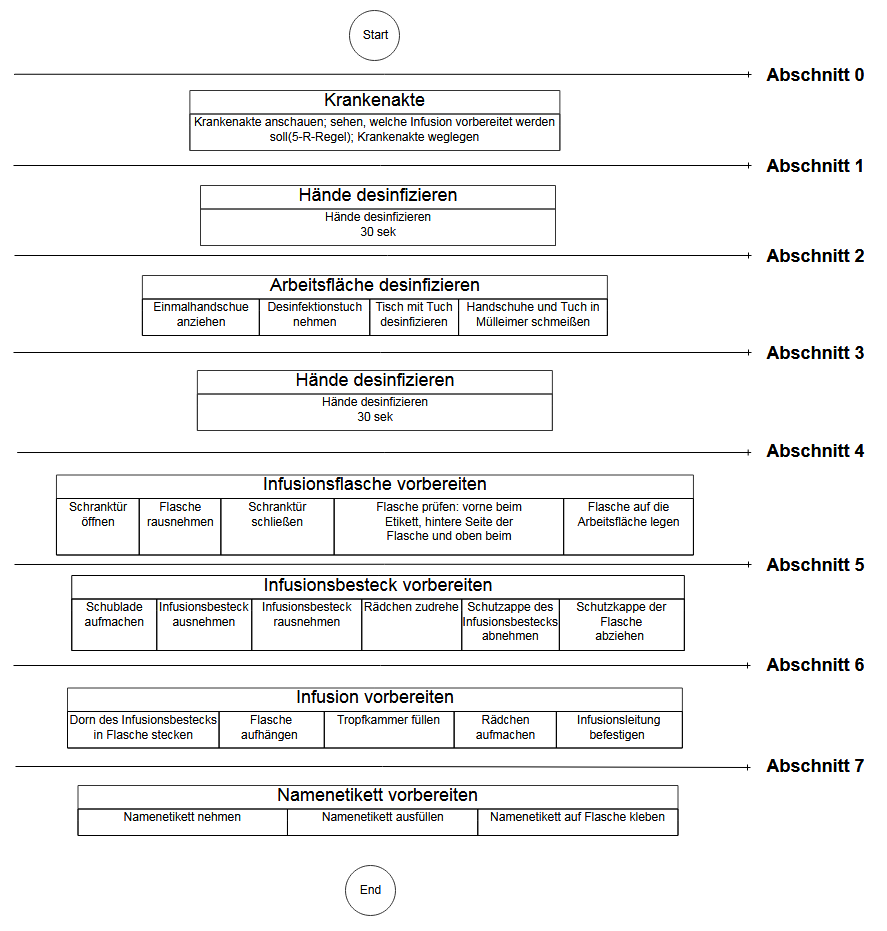
\includegraphics[width=\textwidth]{images/AblaufInfusionsvorbereitung.png}
\caption{Ablauf der Infusionsvorbereitung}
\label{fig:AblaufInfusionsvorbereitung} 
\end{figure}
  
  \subsubsection{Erkennung \& Feedback der Fortschritte}
  Der Fortschritt des Prozesses der Übung wird durch die Durchführung einer richtigen Aktivität gefördert. Wenn eine Aktion des Objektes zur richtigen Zeit durchgeführt wird, wird der Fortschritt erkannt. Die Erkennungen müssen durch die oben genannten Interaktionen nämlich Manipulationen der VR Geräten bewältigt wird. % TODO hier verstehe ich leider nicht, was du meinst :/
  
  Auf dem PC, einem Smartphone und der Gear VR führt eine geeignete Manipulation zu einem Fortschritt. Allerdings ist es bei der HTC Vive anders, weil die 6 DoF Geräte mehr Freiheit bezüglich der Interaktion haben. Zum Beispiel führt das Aufheben eines gefallenen Objektes dzu keinem Fortschritt in der Übung. 
  
  Das Feedback des Fortschritts bietet den Bescheid, dass die aktuelle Aufgabe erledigt wird und die nächste Aufgabe gemacht werden soll. Das Feedbacks wird meistens im Form von Animationen (Translation und Rotation) des Objektes gegeben. Außerdem kann das Feedback durch die Änderung der Eigenschaft (Sichtbarkeit, Farbe) gegeben werden. Zum Beispiel wird ein Haken vor dem Namen dargestellt, wenn der Name von dem Patienten in der Akte überprüft wird.
  
  \subsubsection{Leitung des Ablaufs}
  Der Fortschritt wird durch die richtigen Aktivitäten gefördert. Die Versuche, mit dem richtigen Objekt im falschen Zeitraum oder mit den falschen Objekten zu interagieren, werden ignoriert. Um den Prozess der Übung zu leiten, werden vier Hilfsmitteln angeboten, nämlich das Whiteboard, eine Hinweis-Box, ein 30 Sekunden Indikator und Hacken.
  \begin{itemize}
      \item \textbf{Whiteboard}:
      
      Ein Whiteboard ist auf der linken Wand zu finden, um potentielle Hinweise anzubieten. Wenn eine Aufgabe geschafft wird, wird der Hinweis für die nächste Aufgabe auf dem Whiteboard gezeigt. Wenn sich der Nutzer an dem nächsten Schritt nicht erinnern kann, kann er den Kopf nach links drehen, um den Hinweis zu lesen.
      
      Während der Übung führt keine Aufgabe außer Händedesinfektion zu der Drehung des Kopfs nach links. Das heißt, obwohl der Hinweis dargestellt ist, kann der Benutzer den Hinweis nur durch die absichtliche und bewusste Drehung des Kopfs nach links lesen. Somit wird ein unbeabsichtigtes Lesen vermieden.
      
      \item \textbf{Hinweis-Box}:
      
      Die Hinweis-Box ist ein halb-transparenter Kubus, der in der VR Umgebung dargestellt ist, wenn sich ein Objekt in der Hand befindet.  Die Hinweis-Box hat zwei Funktionen.
      
      Eine davon ist, die Position zu kennzeichnen, wohin das Objekt gelegt werden soll.
      
      Die andere Funktion ist, die Zustände des genommenen Objektes zu zeigen. Wenn ein Objekt gerade in die Hand genommen wird, wird die Hinweis-Box dafür in rot dargestellt. Wenn alle Aufgaben, z.B Überprüfung, zu diesem Objekt erledigt sind, wird die Farbe des Objektes zu grün gewechselt, um den Benutzer zu informieren, dass das Objekt hingelegt werden darf. Wenn das Objekt in der entsprechenden grünen Hinweis-Box hingelegt wird, verschwindet die Hilf-Box und die Position des Objektes wird angepasst. Es gilt, dass das Objekt nicht in die Hinweis-Box positioniert wird, ein Objekt in einer roten Hinweis-Box hinzulegen. (Tabelle ~\ref{tab:HinweisBox}) %TODO da weiß ich auch nicht was du genau meinst :(
      
      \item \textbf{30 Sekunden Indikator}:
      
      Laut fachlicher Anforderung soll die Händedesinfektion 30 Sekunden lang dauern. Um ein eindeutiges Zeichen zu geben, die genaue Zeit darzustellen, wird eine Uhr über dem Armhebelspender mit Händedesinfektionsmittel gehängt. Die Uhrzeit darauf entspricht genau der Zeit in de realen Welt.
      
      Der 30 Sekunden Indikator ist ein roter Halbkreis auf der Platte der Uhr, der genau 30 Sekunden bezeichnet. Wenn der Griff des Armhebelspender gedrückt wird, erscheint der 30 Sekunden Indikator, dessen Ausgangsposition auf dem Sekundenzeiger liegt.
      
      Wenn 30 Sekunden abgelaufen sind, verschwindet der 30 Sekunden Indikator, um den Benutzter damit zu informieren, dass die Händedesinfktion fertig ist und weitere Aufgaben behandeln dürfen.
      
      \item \textbf{Haken}:
      
      Haken bezeichnet die geprüften Elemente, zum Beispiel 5-R bei der Überprüfung der Krankenakte.
  \end{itemize}
  
\begin{table}[]
\resizebox{\textwidth}{!}{%
\begin{tabular}{llll}
\hline
            & Position                                                                         & rot                                                                                                      & grün                                                                                                     \\ \hline
Abschnitt 0 & \begin{tabular}[c]{@{}l@{}}Obere linke\\ Ecke der Arbeitsoberfläche\end{tabular} & Krankenakte in der Hand                                                                                      & 5R überprüft                                                                                             \\ \hline
Abschnitt 2 & Über dem Mülleimer                                                               & Desinfektionstuch in der Hand                                                                                & Arbeitsoberfläche desinfiziert                                                                           \\ \hline
Abschnitt 4 & Auf der Arbeitsoberfläche                                                        & Infusionsflasche in der Hand                                                                                 & Infusionsflasche überprüft                                                                               \\ \hline
Abschnitt 5 & Auf der Arbeitsoberfläche                                                        & Infusionsbesteck in der Hand                                                                                 & Infusionsbesteck überprüft                                                                               \\ \hline
Abschnitt 6 & \begin{tabular}[c]{@{}l@{}}Unter dem Hacken\\ der Infusion Stand\end{tabular}    & \begin{tabular}[c]{@{}l@{}}Infusionsflasche mit\\ eingestochenem Infusionsbesteck\\ in der Hand\end{tabular} & \begin{tabular}[c]{@{}l@{}}Infusionsflasche mit\\ eingestochenem Infusionsbesteck\\ in der Hand\end{tabular} \\ \hline
Abschnitt 7 & Auf der Infusionsflasche                                                         & Namenetikett in Hand                                                                                     & Nameneitkett ausgefüllt                                                                                  \\ \hline
\end{tabular}
}
\caption{Nutzung der Hinweis-Box}
\label{tab:HinweisBox}
\end{table}

  
\subsection{Zusammenfassung}
Webbasierte Applikationen wie LMS sind weit verbreitet. Der Browser kann aus der Sicht der webbasierten Anwendung sogar als mini-Betriebssystem gelten. Deshalb besetzt die WebVR Applikation den unersetzbaren Vorteil, barrierefrei sich in anderen webbasierten Applikation zu integrieren.

Das immersive Erlebnis wird durch die lebendige Umgebung und interaktive Möglichkeiten angeboten. Mit aktueller WebVR Technik sind die visuellen und auditiven Simulationen realisierbar.

Als eine Anwendung einer cross-plattform Technik muss die Konzeption mit unterschiedlichen Geräten gerechnet werden, um bessere Erreichbarkeit zu erreichen. Außerdem werden die individuellen Merkmale der Geräte ausgenutzt, um die bestmögliche Immersion zu erzielen.

Als Lernmaterial werden die VR Übungen die fachlichen Kenntnisse vermitteln. Durch technische Lösungen wird das Verhältnis des Benutzers geleitet, um die richtige Handlung durchzuführen.

Als eine neue Lernmethode wird VR-Training bei E-Learning eine unersetzbare Rolle spielen.

